\chapter{Development}

The result of this research was the development of |miq|, a package manager and
build system for Linux.

miq is a single-file executable that handles the full lifecycle of the build
process of the packages it manages. This stages include:

\begin{enumerate}
    \item Evaluating the expressions that describe packages
    \item Calculating the dependency graph
    \item Fetching the necessary source code
    \item Performing the described build process
    \item Handling the storage and tracking of the installed packages
\end{enumerate}

Therefore, the following sections will all the components that make up miq, and
their interactions.

\section{High level overview}

The development of miq aimed for a modular design, such that
each component didn't have much coupling with the others.
This allows for easy refactoring of parts of the source
code, while leaving the rest of the system untouched. As
such the components of miq can be layed out in figure
\ref{fig:miq-components} .

\begin{figure}[hbtp]
    \centerfloat
    % 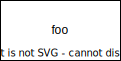
\includegraphics{assets/overview.png}
    \includesvg[width = 450pt]{assets/overview.svg}
    \caption{Overview of the subsystems of miq}
    \label{fig:miq-components}
\end{figure}

Miq is presented as a pipeline of stages, where each
subsystem transform the input data to achieve a desired
state. This design is inspired by other package managers,
which present a similar structure of stages. The main
difference, is that miq works on static package definitions
layed out in a file, which describe the desired state of the
system. In contrast to other package managers, like |apt|,
where the final state of the system is a succession of
commands executed in the shell.

On of the main differences of miq to other package managers,
is how the files are layed out in the filesystem. This is
because each package is given a unique identifier, which in
turns is used for the directory where the package will be
located. This identifier is also unique between different
versions of the same package. And not only that, but it also
encodes the recipe used to build the package itself, and all
of its parents.

To accomplish the tagging of each package with an unique
identifier, a flow of data from package input to package is
visualized on figure \ref{fig:hash}. From a |PackageInput|,
a unique hash is generated, that is the result from hashing
all the fields of the struct. Finally, the hash (an unsigned
32-bit integer) is encoded into text, to form the name of
the package. For this application, the algorithm used is the
\textit{Fowler-Noll-Vo} hash function, which is implemented
in the |fnv| create \cite{FnvRust} . This hash function is
not cryptographically secure, but this was not one of the
design requirements of miq (and can be swapped out for any
other hashing algorithm as needed, as long as it conforms to
the |Hash| trait in Rust).



\begin{minted}{rust}
#[derive(Hash)]
struct PackageInput {
    name: String,
    version: Option<String>,
    script: MetaTextInput,
    deps: Option<Vec<Unit>>,
    env: Option<BTreeMap<String, MetaTextInput>>,
}
\end{minted}

\begin{figure}[hbtp]
    \centerfloat
    \includesvg[width = 0.7\paperwidth ]{assets/hash.svg}
    \caption{Overview of the hashing algorithm}
    \label{fig:hash}
\end{figure}

The implications of this design is that any package gets a
different place on the filesystem, which is derived from
everything that defines the package itself - its build
script and its dependencies, which in turn are also hashed
by the same rules. The advantage of this design, is that
every package has its dependencies perfectly defined,
instead of relying on automatic detection. Let's say that
package |foo| depends of package |bar|. On a conventional
package manager, if |bar| is changed in any form (for
example, updated), then |foo| is usually not modified. But
in essence, now |foo|, if we consider it as a whole, that is
its whole dependency tree, it has changed. This poses a big
issue for the reproducibility of an operating system. Is
|foo| the same if we swapped |bar| for a different version?
Or if we swapped one of |bar|'s dependencies? (Figure
\ref{fig:depswap}) In miq, it is clear that the packages are
no longer the same, as the hashes of its entire dependency
tree has changed, and therefore the name of the output
package. This means that a package "foo" does not really
exist in miq, but rather a package "foo" with a specific hash.

\begin{figure}[hbtp]
    \centerfloat
    \includesvg[width = 200pt]{assets/depswap.svg}
    \caption{Change of dependencies for a package for a conventional package manager}
    \label{fig:depswap}
\end{figure}

% insert depswap-miq.svg
\begin{figure}[hbtp]
    \centerfloat
    \includesvg[width = 200pt]{assets/depswap_miq.svg}
    \caption{Change of dependencies for a package for miq}
    \label{fig:depswap_miq}
\end{figure}

\FloatBarrier
\section{Graph-based dependency resolution}

In software deployment, one of the main goals is to have be
able to reproduce a deployment environment as reliably as
possible. This means that any external factors should be
reduced to a minimum, such that the end result is as close
to the expected as possible. The reality of system
deployments is that not all environments are the same, such
that the same deployment can be applied to different systems
with different hardware -- for example, different network
cards, hard drives or even different architectures.

On the software side, the same problem exists. Any
deployment is composed of different parts of software which
interact with each other. To reduce any external factors,
a possible solution is to try to control the entire software
stack -- from the kernel, to the operating system and
libraries and finally to the application to be deployed.
This can be seen in the deployment of an entire \ac{VM}, that
contain the specific OS required for the application. But
this is not always possible, for example in a managed
environment from a cloud provider. Or it may not be desired
for the cost of implementation and maintenance. One of the
most popular solution nowadays is the use of containers
\cite{DockerAcceleratedContainerized2022}. A container is a
collection of files packaged into an \textit{image}, which is
run by a \textit{container runtime}. The runtime is able to
isolate the main process of the container by using special
Linux capabilities, such as \textit{namespaces}
\cite{NamespacesLinuxManualb}. By isolating the ``child''
process from the host, the container is able to bundle its
entire dependency tree without conflicts with the host.

What is proposed in this project is the usage of the hashing
techniques discussed in the previous section to achieve
isolation of the dependency tree of a child process from the
host. Each file which lives in the miq store, has a unique
path according to its hash.

\begin{minted}{text}
gcc-e3591c92b6d130e5        =>  /miq/store/gcc-e3591c92b6d130e5
bootstrap-5f87f2800c8c639e  =>  /miq/store/bootstrap-5f87f2800c8c639e
\end{minted}

For this reason, a runtime to isolate a process (what is
done with containers) is not needed. Instead, each process
can directly reference the absolute path to the exact
dependency in the store. If package A requires dependency B,
it does not matter if the host \ac{OS} uses also B. If it is
a different version, it will be reflected on its hash -- and
path. If it is exactly the same package B, then the
dependency will be able to be shared across the applications.

\begin{figure}[hbtp]
    \centerfloat
    \includesvg[width=250pt]{assets/depshare.svg}
    \caption{Dependency sharing between applications.}
    \label{fig:dep_share}
\end{figure}

As figure \ref{fig:dep_share} shows, if a there is a
dependency A which is used by two applications, if A is not
the same, the will be no conflict in the file system, as it
will use a different path. By using this technique, we are
able to share the dependencies of multiple application
without the need for containers or namespaces, towards a
more ``native'' approach.

\begin{minted}{text}
identifier => id+hash          => path
A-1.0.0    => A-1.0.0-1f0d1c2b => /miq/store/A-1.0.0-1f0d1c2b
A-1.0.1    => A-1.0.1-a2b3c4d5 => /miq/store/A-1.0.1-a2b3c4d5
A-2.0.0    => A-2.0.0-1f0d1c2b => /miq/store/A-2.0.0-1f0d1c2b
\end{minted}

For the sake of simplicity, the result hash is stripped of
identifiers. Internally, these hashes would be tracked by
the package manager. But for the representation of the
dependency graphs, they are assumed to be computed by miq,
but not displayed. As said in previous sections, the design
decision of tracking each package with a unique hash,
implies that when a node is displayed with a name ``A'', it
is a unique package based on its dependencies and definition
of the package itself.

The data structure used to represent the dependency graph of
a given node ``N'', is a \acl{DAG}. A directed graph
consists of a non-empty finite set of elements called nodes
and a finite set of ordered pairs of distinct nodes called
edges. A directed graph with no cycles is called a \ac{DAG}
\cite{bang-jensenDigraphs2009} . The representation of this
is simply a list of nodes and edges such as the following.

\begin{figure}[hbtp]
    \centering
    \begin{minipage}[t]{0.5\textwidth}

    \begin{minted}{dot}
        digraph G {
          // Nodes
          a;
          b;
          c;
          // Edges
          a -> b;
          a -> c;
          b -> c;
        }
    \end{minted}
    \end{minipage}
   \caption{\texttt{dot} language for describing graphs.}
   \label{fig:dot_graph}
\end{figure}

\begin{figure}[hbtp]
    \centerfloat
    \includesvg[width=70pt]{graph/sample.dot.svg}
    \caption{Resulting visualization for the graph in figure \ref{fig:dot_graph}.}
\end{figure}

For a generic \ac{DAG}, we can define the nodes and edges as
``weighted''. A weight is a value attached to the element.
Common examples of weighted nodes are ``labels'' -- like
|a,b,c| in figure \ref{fig:dot_graph} -- numeric values,
that can represent a cost or a distance, depending on the
application of the graph. Edges can also be weighted, with
also the common use of numeric values. For the topic of
package management, on first instance the edges are not
weighted -- or implemented as a |null| value. The nodes then
can represent an identifier for a package. Because in the
miq software deployment model, we can identify a package by
its path in the store
(|/miq/store/<name>-<version>-<hash>|), a node weight can be
represented just by a |String| type in Rust. Therefore, the
edge directions represent a dependency between two packages,
read like:

\begin{minted}{text}
"A depends on B"
 A    ==>     B
\end{minted}

For the purpose of this application, the term "to depend on"
is flattened over any type of dependency. Instead of
specifying whether a dependency occurs at ``runtime'' or
``buildtime'', this is simplified to just ``depend''. An
example of how dependencies can be split into different
categories is present in \textit{Gentoo's Ebuild system}
\cite{DependenciesGentooDevelopment}. In Gentoo,
dependencies are split in 3 categories: |BDEPEND| (required
at build-time in the build machine), |DEPEND| (required at
build-time, for the target machine) and |RDEPEND| (required
at run-time, for the target machine) (figure \ref{fig:dep_categories} ). Many Linux
distributions implement the same 3 variants, with different
naming conventions. What this allows it stripping packages
once the package has been built. This is specially useful on
binary-based distributions, where you don't need to
distribute the compiler for a package, but only its
link-time dependencies and run-time dependencies. As noted
before, these differences are not considered in miq, and
just a generic ``dependency'' is used for both run-time and build-time.

\begin{figure}[hbtp]
    \centerfloat
    \begin{tabular}{lll}
        \hline
        & Build-time & Run-time \\
        \hline
        Build machine & |BDEPEND| & - \\
        Target machine & |DEPEND| & |RDEPEND| \\
        \hline
    \end{tabular}
    \caption{Dependency categories in Gentoo \cite{DependenciesGentooDevelopment} .}
    \label{fig:dep_categories}
\end{figure}

Finally, one of the properties of a \ac{DAG} is that there
is always an acyclic ordering of the nodes
\cite{bang-jensenDigraphs2009}. This means, that we can get
an ordered list of all the nodes starting from a root node,
without cycles. A cycle in package management is an
undesirable entity. What it is translated to, is that ``a
package depends on itself''. For a binary based
distribution, this is not a hard problem to solve, as the
packages are usually applied into the system in any order.
But for a source-based distribution, a cycle in the
dependency graph is impossible to solve: to be able to build
a package, we require the package itself as an input,
leading to a paradox. This is usually solved by introducing
multiple ``intermediate'' packages -- for example, a package
A without less features, such that it doesn't depend on
itself.

The usage of a \ac{DAG} is also very useful to represent the
dependencies in a manifest on disk. As instead of committing
multiple actions into the live system, a manifest can be
used to declare all dependencies front-loaded.

In the following sections, it is described how the dependency
graphs are implemented in miq, and how they are used to walk
the dependency tree to build all packages in parallel.

\begin{figure}[hbtp]
    \centerfloat
    \includesvg[width=0.7\paperwidth]{graph/libc.dot.svg}
    \caption{Dependency graph for the package
    \texttt{stage0.libc}, hashes stripped.}
    \label{fig:m4_graph}
\end{figure}

\subsection{Immutability}

To build reliable system deployments, it is important to reduce the
number of variables that can affect the outcome. From the
software perspective, this means that the system should
either be reliant to changes in the environment, or minimize
the factors from the host that can affect the application.
In Linux, one of the main factors that can affect the
environment are the libraries that are installed on the
system.

On the previous section it was discussed how a different
approach to tagging the packages on the filesystem can be
used to achieve a consistent environment. What this
filesystem layout naturally leads into, is a system where
there is no mutation of the existing packages. On a
classical system, to upgrade a package, the following steps
are taken:

\begin{enumerate}
    \item Download the new update for package |foo|, and unpack it
    \item Replace file |/usr/bin/foo| with the new version
    \item Replace file |/usr/share/foo-bar| with the new version
    \item \ldots
    \item Register the new version in the database
\end{enumerate}

As can be seen, the process of upgrading a package involves
multiple in-place modifications of the existing package.
This operation can be qualified as ``surgical'', as it may
involve many operations which can fail -- and always
eventually fail. A failure in the middle of a upgrade
process can leave the system on a inconsistent state.

\begin{enumerate}
    \item Download the new update for package |foo|, and unpack it
    \item Replace file |/usr/bin/foo| with the new version
    \item Failed to upgrade |/usr/share/foo-bar|, aborting
\end{enumerate}


\subsection{Atomicity}


\subsection{Stages}



\subsection{ELF format}

\subsection{The bootstrapping problem}

\subsection{libc}

\section{Builder}

\section{Graph evaluator}

\section{Lua evaluator}

\section{Other components}

